\documentclass[aspectratio=169]{beamer}
\usetheme{Madrid}
\usepackage{tikz}
\usetikzlibrary{positioning, arrows.meta}
\usepackage{booktabs}

\title{\texorpdfstring{Ensemble of Agents --- Class 1}{Ensemble of Agents - Class 1}}
\subtitle{\texorpdfstring{DSC 180A, Fall 2026 \quad Domain D31}{DSC 180A, Fall 2026, Domain D31}}
\author{Yoav Freund}
\institute{UC San Diego}
\date{Fall 2026}

\setbeamertemplate{navigation symbols}{}

\begin{document}

% 1
\begin{frame}
  \titlepage
\end{frame}

% 2
\begin{frame}{Administration: GitHub}
  \begin{itemize}
    \item Email your GitHub username to \texttt{yfreund@ucsd.edu}
    \item You will be added to the course repo: \textbf{[repo URL]}
    \item All code, reports, and experiment logs live in the repo
  \end{itemize}
\end{frame}

% 3
\begin{frame}{Administration: WhatsApp}
  \begin{itemize}
    \item Join the group: \textbf{[WhatsApp link]}
    \item WhatsApp: scheduling, quick questions
    \item GitHub: code, issues, decisions
  \end{itemize}
\end{frame}

% 4
\begin{frame}{Components of a learning system}
  \centering
  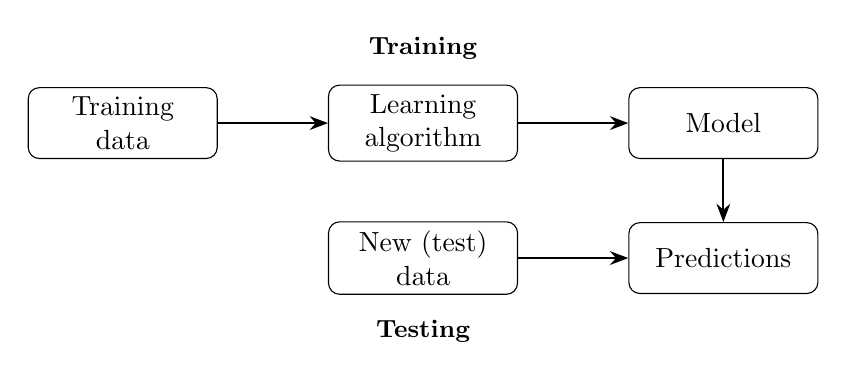
\begin{tikzpicture}[
    node distance=0.8cm and 1.4cm,
    box/.style={draw, rounded corners, minimum width=2.4cm, minimum height=0.9cm, align=center},
    arr/.style={-Stealth, thick}]
    \node[box]                     (train) {Training\\data};
    \node[box, right=of train]     (alg)   {Learning\\algorithm};
    \node[box, right=of alg]       (model) {Model};
    \node[box, below=of model]     (pred)  {Predictions};
    \node[box, left=of pred]       (new)   {New (test)\\data};
    \draw[arr] (train) -- (alg);
    \draw[arr] (alg) -- (model);
    \draw[arr] (new) -- (pred);
    \draw[arr] (model) -- (pred);
    \node[above=0.2cm of alg, font=\small\bfseries] {Training};
    \node[below=0.2cm of new, font=\small\bfseries] {Testing};
  \end{tikzpicture}

  \vspace{0.6cm}
  \begin{itemize}
    \item Training produces a model
    \item Testing runs the model on data it has not seen
  \end{itemize}
\end{frame}

% 5
\begin{frame}{What testing measures}
  \begin{itemize}
    \item \textbf{Accuracy:} error rate on new data
    \item \textbf{Confidence:} does the model know when it may be wrong?
    \item \textbf{Speed:} time per prediction
  \end{itemize}
\end{frame}

% 6
\begin{frame}{Inference: throughput and latency}
  \begin{itemize}
    \item \textbf{Latency:} time to answer one request
    \item \textbf{Throughput:} requests answered per second
  \end{itemize}
  \vspace{0.3cm}
  \begin{columns}[T]
    \column{0.35\textwidth}
    \centering
    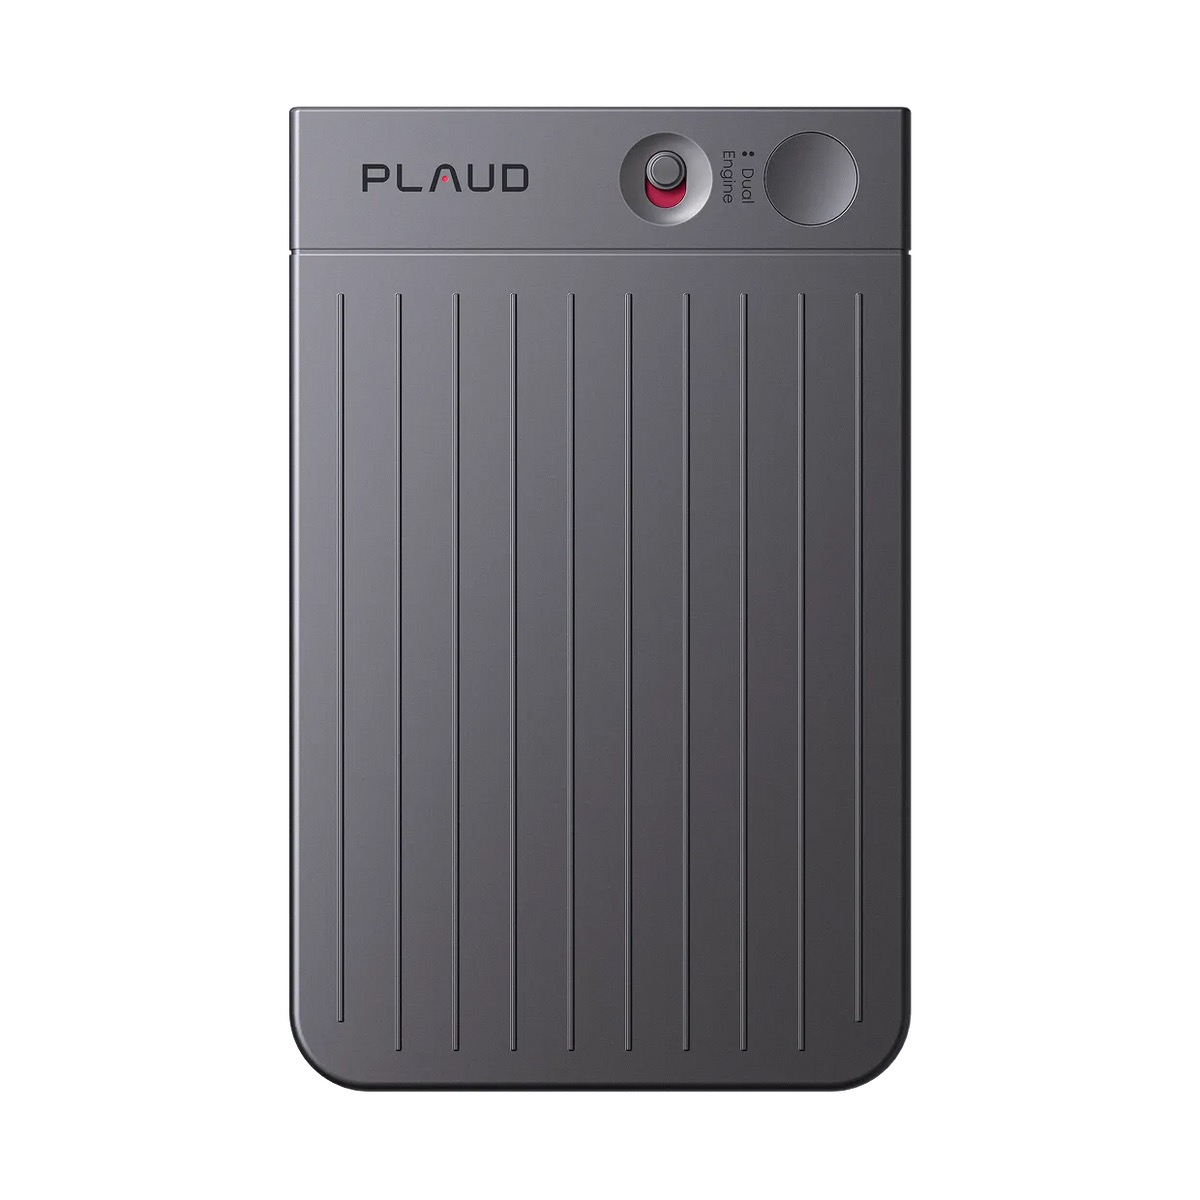
\includegraphics[height=4cm]{images/plaud-note.jpg}\\
    {\tiny Plaud Note. Image: plaud.ai (editorial use)}
    \column{0.6\textwidth}
    \begin{itemize}
      \item Pocket speech recognizers are too small for large speech models
      \item Audio is recorded on the device, then sent to the cloud for transcription
      \item Cost of the cloud:
      \begin{itemize}
        \item network delay
        \item needs connectivity
        \item privacy
        \item per-minute fees
      \end{itemize}
    \end{itemize}
  \end{columns}
\end{frame}

% 7
\begin{frame}{The agent loop}
  \begin{columns}[T]
    \column{0.36\textwidth}
    \small
    \begin{itemize}
      \item An agent is an LLM in a loop: read goal and context, decide, call a tool, observe, repeat
      \item \textbf{Tools:} run code, read/write files, search, call another agent
      \item \textbf{Memory:} the growing context of actions and observations
      \item In this course: learner agents train models; a coordinator agent runs the loop over them
    \end{itemize}
    \column{0.64\textwidth}
    \centering
    \vspace{0.4cm}
    \scalebox{0.85}{%
    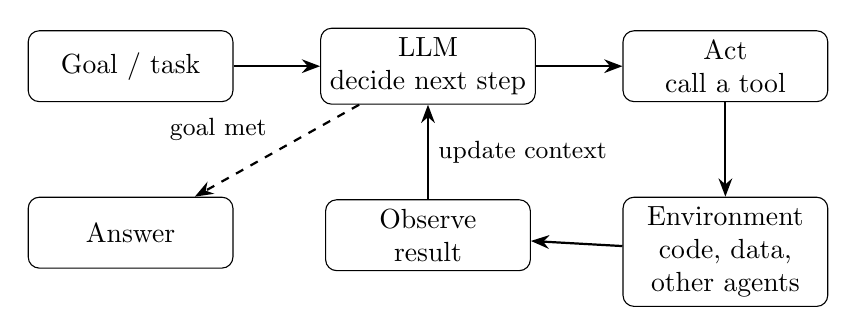
\begin{tikzpicture}[
      node distance=1.2cm and 1.1cm,
      box/.style={draw, rounded corners, minimum width=2.6cm, minimum height=0.9cm, align=center},
      arr/.style={-Stealth, thick}]
      \node[box]                  (goal)  {Goal / task};
      \node[box, right=of goal]   (think) {LLM\\decide next step};
      \node[box, right=of think]  (act)   {Act\\call a tool};
      \node[box, below=of act]    (env)   {Environment\\code, data,\\other agents};
      \node[box, below=of think]  (obs)   {Observe\\result};
      \node[box, below=of goal]   (done)  {Answer};
      \draw[arr] (goal) -- (think);
      \draw[arr] (think) -- (act);
      \draw[arr] (act) -- (env);
      \draw[arr] (env) -- (obs);
      \draw[arr] (obs) -- node[right, font=\small]{update context} (think);
      \draw[arr, dashed] (think) -- node[above left, font=\small]{goal met} (done);
    \end{tikzpicture}}
  \end{columns}
\end{frame}

% 8
\begin{frame}{The agent loop as a learning system}
  \begin{columns}[T]
    \column{0.35\textwidth}
    \textbf{Agent loop}
    \begin{itemize}
      \item LLM
      \item Tools
      \item Observation
      \item Goal
    \end{itemize}
    \column{0.6\textwidth}
    \textbf{Learning system}
    \begin{itemize}
      \item Training: choose method and next update
      \item Calculate error, gradient, latency
      \item Error, gradient, and latency values
      \item Good performance on the test set
    \end{itemize}
  \end{columns}
  \vspace{0.6cm}
  \begin{alertblock}{Caution}
    The agent sees only training and validation data; the test set is used once, at the end.
  \end{alertblock}
\end{frame}

% 9
\begin{frame}{Ensembles of agents}
  \begin{itemize}
    \item Sometimes it is useful to break the learning task into smaller learning tasks and combine the results
    \item Ensembles work that way
    \item Each small task goes to its own learner agent; a coordinator agent combines their predictions
  \end{itemize}
  \vspace{0.3cm}
  \centering
  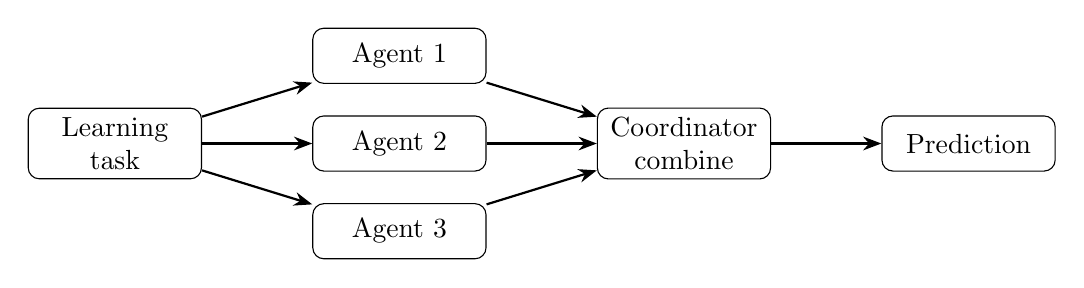
\begin{tikzpicture}[
    node distance=0.4cm and 1.4cm,
    box/.style={draw, rounded corners, minimum width=2.2cm, minimum height=0.7cm, align=center},
    arr/.style={-Stealth, thick}]
    \node[box]                    (task) {Learning\\task};
    \node[box, right=of task]     (a2)   {Agent 2};
    \node[box, above=of a2]       (a1)   {Agent 1};
    \node[box, below=of a2]       (a3)   {Agent 3};
    \node[box, right=of a2]       (comb) {Coordinator\\combine};
    \node[box, right=of comb]     (pred) {Prediction};
    \foreach \a in {a1,a2,a3} {
      \draw[arr] (task) -- (\a);
      \draw[arr] (\a) -- (comb);
    }
    \draw[arr] (comb) -- (pred);
  \end{tikzpicture}
\end{frame}

% 10
\begin{frame}{Examples of ensembles}
  \begin{itemize}
    \item \textbf{Bagging} (Breiman 1996): train many learners on bootstrap samples; majority vote
    \item \textbf{Random forests} (Breiman 2001): bagging of trees, each split chosen from a random subset of features
    \item \textbf{Boosting} (Freund and Schapire 1997): train learners in sequence, each focusing on the examples the previous ones got wrong; weighted vote
    \item \textbf{Decision trees!} Each split breaks the task into smaller learning tasks on subsets of the data; each leaf solves its own small task. Divide and conquer, rather than vote
  \end{itemize}
\end{frame}

% 11
\begin{frame}{Week-by-week plan}
  One student per week: present a paper (with slides), implement it or find an implementation, and run it on a Kaggle dataset. Report accuracy, confidence, and speed.

  \vspace{0.4cm}
  \centering
  \small
  \begin{tabular}{llll}
    \toprule
    Week & Method & Paper & Presenter \\
    \midrule
    2 & Averaged perceptron & Freund and Schapire (1999) & Andrew Chen \\
    3 & Bagging & Breiman (1996) & Saisohan Shingade \\
    4 & Random forests & Breiman (2001) & Surya Setty \\
    5 & Boosting stumps & Freund and Schapire (1997) & Uday Lingampalli \\
    \bottomrule
  \end{tabular}

  \vspace{0.4cm}
  \raggedright
  \footnotesize Freund and Schapire (1999): ``Large margin classification using the perceptron algorithm.'' Students may swap weeks among themselves.
\end{frame}

\end{document}
